\chapter{Second Use Case: Music Recommender System}
\graphicspath{{Chapter09/Figures/}}
\label{chap:challenge}

In recent years, music streaming services strongly modified the way in which people access to music content. In particular, the music experience does not foresee anymore to follow pre-defined collections of tracks edited by music artists or labels: the end-user is now free to produce her own playlist with potentially unlimited freedom. As a consequence, the automatic playlist generation and continuation are now crucial tasks in the recommender system field.

This chapter describes the results obtained by the D2KLab team, lead by the author of this dissertation, for the task of playlist completion obtained in the context of the RecSys Challenge 2018. This work relies on an ensemble strategy which involves different types of features, including sequential embeddings, title embeddings and lyrics features. Therefore, the proposed approach could be considered a multicriteria sequence-based recommender system. Following the challenge rules,\footnote{\url{https://recsys-challenge.spotify.com/rules}} the target dataset is the Million Playlist Dataset (MPD), which contains metadata for 1 million playlists gathering more than 2.2 million distinct tracks. The implementation of our approach is publicly available on GitHub.\footnote{\url{https://github.com/D2KLab/recsys18_challenge}}

The remainder of this chapter is structured as follows: Section~\ref{rnn:sec:ensemble} presents our ensemble approach, while Section~\ref{rnn:sec:rnn} details the design of the Recurrent Neural Networks. In Section~\ref{rnn:sec:t2r} we discuss the intuition behind the implementation of Title2Rec. Section~\ref{rnn:sec:optimization} explains the optimization conducted on the ensemble, the RNN, and Title2Rec. We describe the experimental results in Section~\ref{rnn:sec:results}. Finally, in Section~\ref{rnn:sec:conclusion}, we provide the conclusions.

\section{Ensemble}
\label{rnn:sec:ensemble}

Our approach builds upon an ensemble voting strategy of different runs of multiple Recurrent Neural Networks (RNNs) and one execution of Title2Rec. The RNNs are configured differently in terms of network inputs and hyper-parameters. The RNNs are used to predict the missing tracks to be part of a playlist and thus assume to have seed(s) track(s) of the playlist to be utilized as initial elements of the network bootstrap (Section~\ref{rnn:sec:rnn}). However, when only the title of the playlist is available, our approach relies on a fall-back strategy that implements a K-means clustering of the playlists and a word embedding model of their titles (trained with fastText), called Title2Rec (Section~\ref{rnn:sec:t2r}). Figure~\ref{rnn:fig:ensemble} illustrates the overall approach.

\begin{figure}
\centering
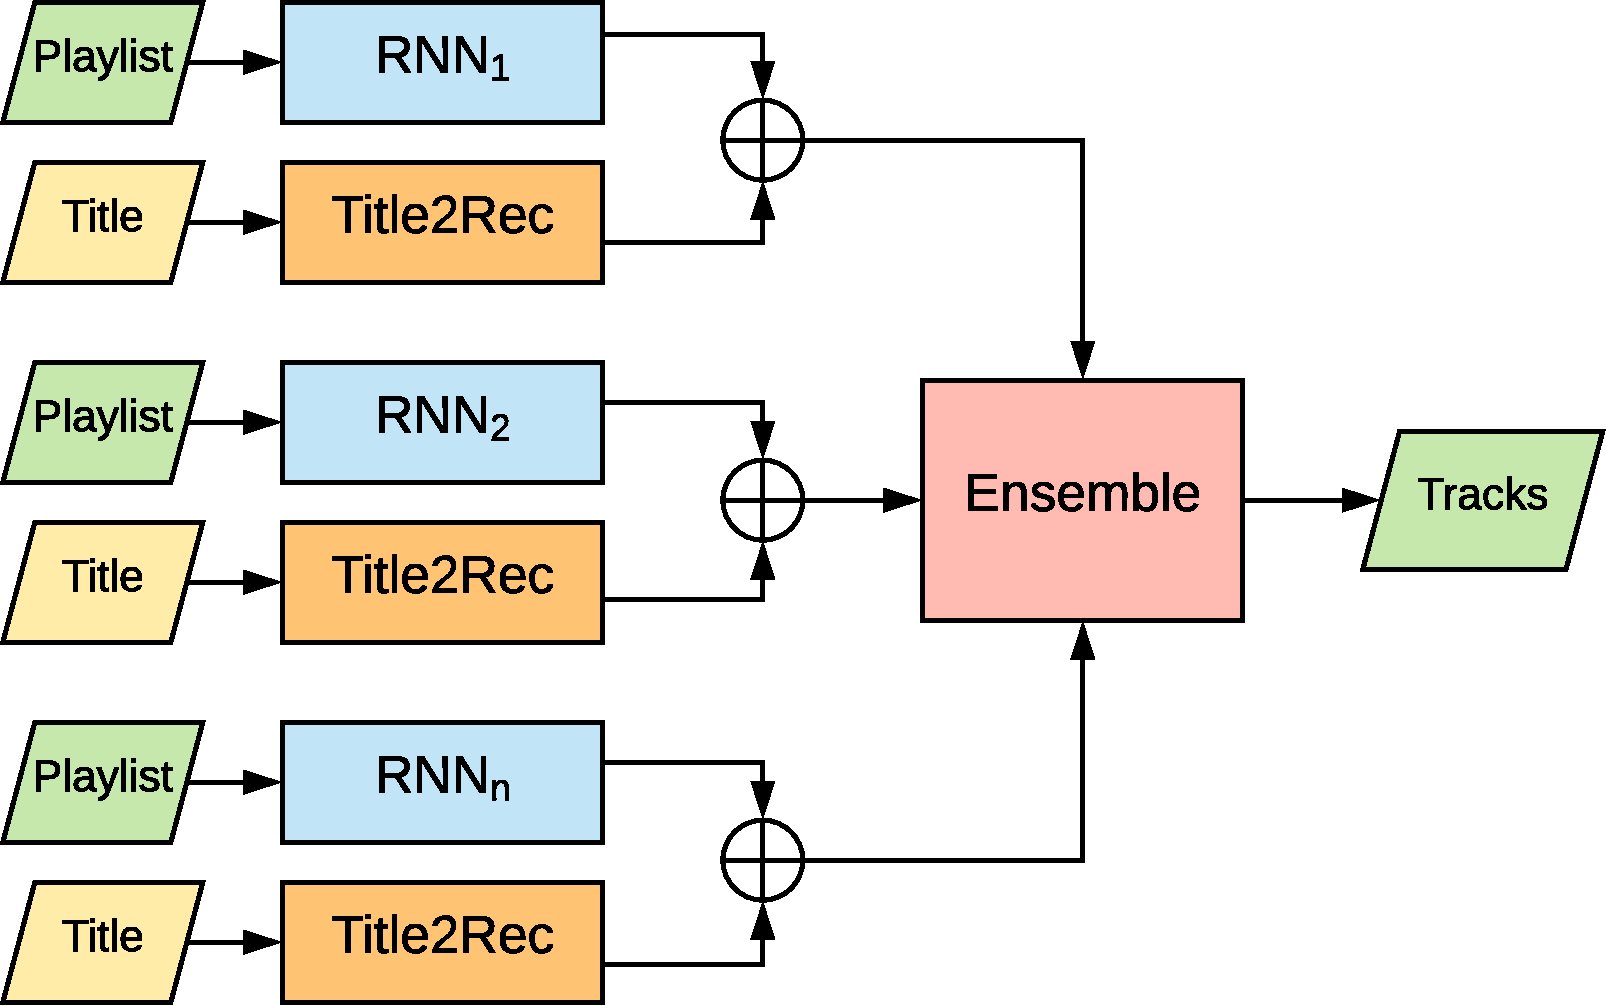
\includegraphics[width=\textwidth, width=0.75\textwidth]{ensemble}
\caption[Ensemble architecture for playlist completion]{The proposed ensemble architecture for playlist completion. The inputs are a playlist and its title.}
\label{rnn:fig:ensemble}
\end{figure}

The ensemble weighs the rankings of the different runs by giving more importance (more weights) to the top ranked tracks and less to the low ranked tracks, similarly to a Borda count election. In detail, given a ranked set of predictions coming from a configuration $k$, corresponding to a particular configuration of the RNN jointly combined with Title2Rec, $R_k = \{T_1, T_2, \dots, T_{500}\}$, we assign to each track a score $s_k$ that has its maximum for the first track in the ranking and minimum for the last one, i.e. $s_k(T_i) = 500 - i + 1$. Then, we sum the scores over all the configurations that we want to ensemble, obtaining a final score for each track $s(T_i) = \sum_{k} s_k(T_i)$ that we use to create the final ranking of the tracks. Take as an example (with 3 tracks instead of 500 in the predictions) a configuration $1$ with ranking $R_1 = \{T_1, T_2, T_3\}$ and a configuration $2$ with ranking $R_2 = \{T_1, T_3, T_2\}$. We would get $s_1(T_1) =  3$, $s_1(T_2) = 2$, $s_1(T_3) = 1$, $s_2(T_1)=3$, $s_2(T_3) = 2$, $s_2(T_2)=1$ and thus $s(T_1) = 3+3= 6$, $s(T_2)= 2+1=3$, $s(T_3)=1+2=3$, obtaining as a final ranking $R = \{T_1, T_2, T_3\}$, or equivalently $R = \{T_1, T_3, T_2\}$ as $T_2$ and $T_3$ have the same score.

\section{Recurrent Neural Networks}
\label{rnn:sec:rnn}

Recurrent Neural Networks (RNNs) are one of the most commonly used typology of neural networks~\cite{Lecun2015}. In recent years, thanks to advancements in their architecture~\cite{Hochreiter1997,Chung2014} and in computational power, they have become the standard to effectively model sequential data. They have been used successfully for tasks such as sentiment analysis~\cite{Tang2015}, speech recognition~\cite{Graves2013}, image captioning~\cite{Karpathy2015}, predicting tourist paths~\cite{Palumbo2017} and neural language models~\cite{Mikolov2010}. One of the typical applications of RNNs is language modeling, i.e. the task of learning a probabilistic model of text in order to generate new text by recursively predicting the next word in a sentence~\cite{Sutskever2011}. We use RNNs, more specifically Long-Short Term Memory (LSTM) cells~\cite{Hochreiter1997}, in a similar vein to the language modeling problem, i.e. training the network to predict the next track in a playlist and sampling tracks from the learned probability model to generate predictions. In practice, rather than using only the track as input, we use a richer representation that also exploits the artist, the album, the title and, possibly, lyrics features (Figure~\ref{rnn:fig:global_architecture}). 

In the following sections, we describe in detail the input features as well as the generation strategy.

\begin{figure}
\centering
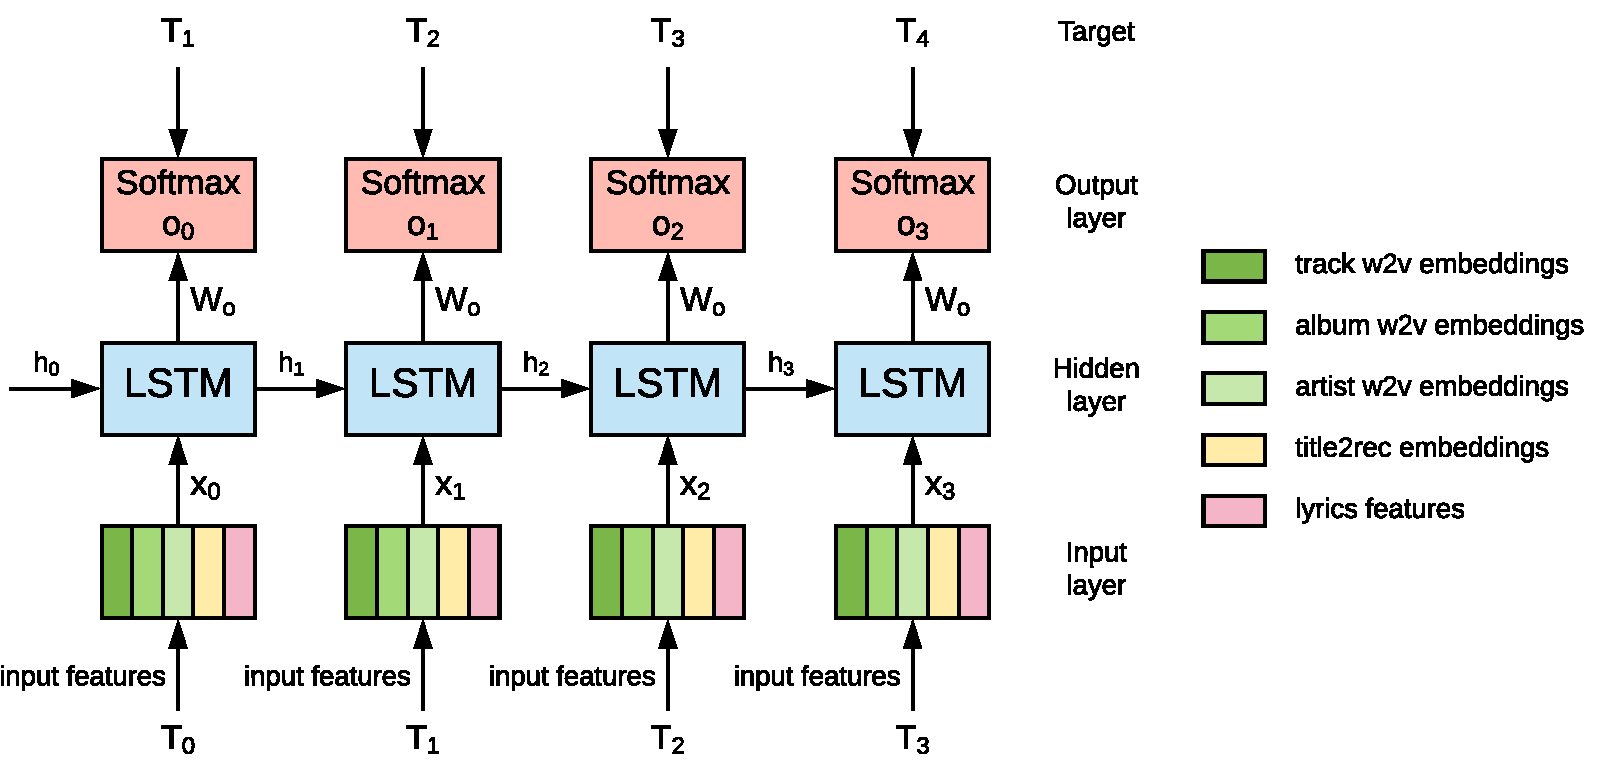
\includegraphics[width=\textwidth]{rnn}
\caption[RNN architecture for playlist completion]{Our RNN architecture for playlist completion. The input vectors include word2vec embeddings for the track, the album, and the artist, a fastText embedding for the playlist title and numerous features extracted from the lyrics.}
\label{rnn:fig:global_architecture}
\end{figure}

\subsection{Input Vectors}

\subsubsection{Track, Album and Artist Embeddings}
\label{rnn:sec:track_embs}

In order to leverage the information in the dataset concerning tracks, artists and albums, we opt for an approach based on word2vec~\cite{Mikolov2013} embeddings. More precisely, we train the word2vec model separately on sequences of tracks, albums and artists in the order of appearance in the playlist, obtaining three separated word2vec models encoding co-occurrence patterns of tracks, albums and artists respectively. Each word2vec model is based on the Skip-gram model with negative sampling using default hyper-parameters of the Gensim implementation~\cite{Rehurek2010}: embedding vector dimension is $d=100$, learning rate $\alpha = 0.025$ linearly decaying up to $min_{\alpha} = 0.0001$, window size $c = 5$, number of epochs is $\eta = 5$.

We concatenate the three representations of the tracks, albums and artists, obtaining an input vector $x_{w2v}$ whose dimensionality is $|x_{w2v}| = 300$.

\subsubsection{Title Embeddings}
\label{rnn:sec:title_embs}

The title of a playlist can potentially contain interesting information about the intention and the purpose of its creator. The title can suggest that the tracks in certain playlist are intended to suit a certain goal (e.g. \textit{party}, \textit{workout}), a mood (\textit{sad songs}, \textit{relaxing}), a genre (\textit{country}, \textit{reggae}), or a topic (\textit{90's}, \textit{Christmas}). Our intuition, supported by the experiments described later in this section, is that playlists with similar titles may contain similar tracks.
The title similarity could rely on pre-trained models and thesauri. However, we opted for computing a model that is specific for the playlist continuation task, using the sole data of the MPD.

A playlist embedding $p_{w2v}$ is computed as the mean of the embeddings of the tracks composing the playlist, as generated in the previous section. The playlist embeddings are then grouped in $n$ clusters, applying the K-means algorithm~\cite{Hartigan1979}.

We empirically observed that, apart from very general clusters, we also created clusters containing specialized playlists, obtaining as a consequence groups of titles that belong to the same semantic area. For example, a cluster contains playlists like \textit{Christmas feels}, \textit{December} or with titles including the emoji of Santa Claus, while another group encompasses playlists like \textit{country} and \textit{Alabama}.

Each cluster $c$ expresses a composed label, which is the concatenation of the titles of all the playlist $p \in c$ separated by a blank space. These labels can be seen as a corpus of $n$ documents (one for each cluster) that is used as input for the fastText algorithm~\cite{Joulin2016}. Because this algorithm is able to represent textual information at the level of n-grams from 3 to 6 character, the Title2Rec model in output computes the embeddings of any playlist title, being this already seen in the dataset or totally unknown. Figure~\ref{rnn:fig:t2r_pipeline} illustrates the process of the Title2Rec model generation.

\begin{figure}
\centering
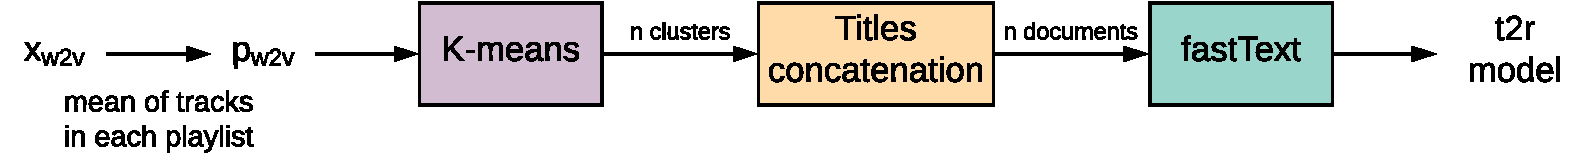
\includegraphics[width=\textwidth]{t2r}
\caption[Pipeline for the title embedding model]{The pipeline for generating the title embedding model used in Title2Rec. The embeddings are computed through a fastText model trained on a corpus of concatenated titles of similar playlists.}
\label{rnn:fig:t2r_pipeline}
\end{figure}

\subsubsection{Lyrics Embeddings}
\label{rnn:sec:lyrics}

Since playlists contain tracks that share semantic properties (such as the genre) and acoustic properties (such as the mood), we hypothesize their lyrics share features as well. To this end, we extract numerous features from the lyrics for a large set of tracks used in the MPD dataset ($v \in \mathbb{R}^{n}$) that describe different stylistic and linguistic dimensions of a song text:

\begin{itemize}
\item \textit{vocabulary} ($v \in \mathbb{R}$): as a measure of the vocabulary richness, we compute the type-token ratio of a song text.
\item \textit{style} ($v \in \mathbb{R}^{27}$): to estimate the linguistic style of a song text, we measure the line lengths (in characters and in tokens) and the frequencies of all major part-of-speech tags. We further count rhyme occurrences and \qu{echoisms} (sung words like \qu{laaalala} and \qu{yeeeeeeeaaaaaaah}).
\item \textit{semantics} ($v \in \mathbb{R}^{60}$): we build a topic model with 60 topics on the song text bag of words using Latent Dirichlet Allocation~\cite{Blei2003}. Each song text is then represented by its association to these topics.
\item \textit{orientation} ($v \in \mathbb{R}^{3}$): this dimension models how the song narrative (entities, events) is oriented with respect to the world. We encode a temporal dimension, i.e. whether the song mainly recounts past experiences or present/future ones, by representing the fraction of past tense verb forms to all verb forms as a feature.
\item \textit{emotion} ($v \in \mathbb{R}^{6}$): we model the subjectivity (subjective vs. objective) as well as the polarity (positive vs. negative) of the song text. Furthermore, the emotions conveyed are modelled in a common two-dimensional model that accounts for degrees of arousal and valence.
\item \textit{song structure} ($v \in \mathbb{R}^{4}$): as a proxy of the structure of the lyrics, we use the line lengths as well as the lengths of paragraphs in the song text.
\end{itemize}

For experimental purposes, we grouped the previous features in two categories:

\begin{itemize}
\item \textit{deterministic} ($v \in \mathbb{R}^{23}$): it encompasses all features generated in a deterministic way such as features related to the structure, the vocabulary, and the style of the lyrics. We excluded from this group the frequencies of part-of-speech tags, as they depend on the tagger used.
\item \textit{fuzzy} ($v \in \mathbb{R}^{18}$): it includes the features generated in a non-deterministic fashion such as orientation, emotion, and the frequencies of POS tags.
\end{itemize}

All features are scaled using a custom feature scaler that combines two elements. It accounts for outliers by scaling the data non-linearly based on the percentile of the feature value distribution they belong to. Finally, it scales the data linearly to the same $[-1,1]$ interval that non-lyrics features live in.

Retrieving lyrics for the MPD dataset is achieved by linking it to the WASABI corpus~\cite{Meseguer2017}.\footnote{\url{https://wasabi.i3s.unice.fr}} The WASABI corpus is an ongoing resource that contains 2.1M song texts (of 77k artists), and for each song it provides the following information: the lyrics extracted from \url{http://lyrics.wikia.com}, the synchronized lyrics (when available) from \url{http://usdb.animux.de}, DBpedia abstracts and categories the song belongs to, genre, label, writer, release date, awards, producers, artist and/or band members, the stereo audio track from Deezer (when available), the unmixed audio tracks of the song, its ISRC, BPM, and duration. In total, we linked 416k tracks in MPD (out of 2.2M unique tracks) to WASABI tracks that contain the lyrics. While the linked tracks proportion with $\sim$20\% seems small, the linked tracks cover 53\% of all 66M track occurrences in MPD because of the typical fat-tailed distribution, where some songs are extremely common while most titles occur only rarely in a playlist. Linking the lyrics was done in three levels of accuracy: direct Spotify URI matching gave us 155k links, exact artist and title matching provided 334k matches, and finally lower casing and deleting bracketed content (in song titles only) led to 51k matches. As the results overlap we ended up with 416k matched tracks in total. Some of our lyrics features are language-specific, so we decided to compute lyrics features exclusively on English song texts. This finally resulted in 367k English song texts we computed lyrical features on. Language detection is done with the \textit{langdetect} package\footnote{\url{https://github.com/Mimino666/langdetect}} and datasets of MPD and WASABI are merged along the axes of their Spotify URIs, artist names, song title names, respectively.

\subsection{Learning Model}

As mentioned earlier, we address the problem of playlist continuation as a language modeling problem. More specifically, we train the RNN to predict the next track in a playlist, defining the targets $Y$ to be the inputs $X$ shifted in time, i.e. $X = \{(\hat{T{^j}}_0, \hat{T{^j}}_1, \dots, \hat{T^{j}}_{N_j -1})\}$ and $Y = \{(T{^j}_1, T{^j}_2, \dots, T^{j}_{N_j})\}$ where $\hat{T}$ represents a track and its metadata (artist, album, playlist title, lyrics features), $T$ represents a track id in a playlist, $j = 1, \dots, M$ is a playlist index and $N_j$ is the length of the j-\textit{th} playlist. In this way, we train the model to learn a probability distribution of the next track $P (T_N | \hat{T}_{N-1}, \hat{T}_{N-2}, \dots, \hat{T}_{0})$ given the previous ones, which is parametrized by the network outputs that are converted into probabilities by the final softmax layer (Figure~\ref{rnn:fig:global_architecture}). The training algorithm attempts to minimize the cross-entropy loss function $L$, that measures the disagreement between the learned probability model and the observed probability model of the targets $Y$. The perplexity metric that is reported in the experiments is similar to the one detailed in Section~\ref{seq:sec:perplexity} and it corresponds to $ppl = 2^{L}$. In practice, rather than using probabilities, we use the `logits' $p_i$ where $i$ is a track index, un-normalized scores that are proportional to the probabilities. Different optimization algorithms to minimize the loss are empirically compared to select the most appropriate one.

\subsection{Generating Predictions}
\label{rnn:sec:generation}

We experiment three different strategies to generate track predictions from the RNN. Given an input seed and the hidden state, the trained model outputs the logits $p_i$, i.e. un-normalized scores that are proportional to the probability that a given track appears after the sequence of seeds $s$. In details, we considered the following approaches, as depicted in Figure~\ref{rnn:fig:predictions}.

\begin{description}[font=\tt]
\item[do\_sample] It samples the track with the highest logit $p_i$, where $\hat{i} = arg\ max ({p_i})$, given the set of seeds $s$. It adds the sampled track $\hat{i}$ to the seeds $s$, then it repeats the previous operations until 500 tracks are sampled.
\item[do\_rank] It ranks the tracks according to their logit value $p_i$, given all the seeds $s$, then it selects the top-500 tracks with the highest logit.
\item[do\_summed\_rank] It computes the logits $p_i$ for every seed. It averages all the logits in the sequence obtaining $\hat{p_i}$ and then it ranks the tracks according to the values of $\hat{p_i}$.
\end{description}

\begin{figure}
\centering
\begin{subfigure}{.8\textwidth}
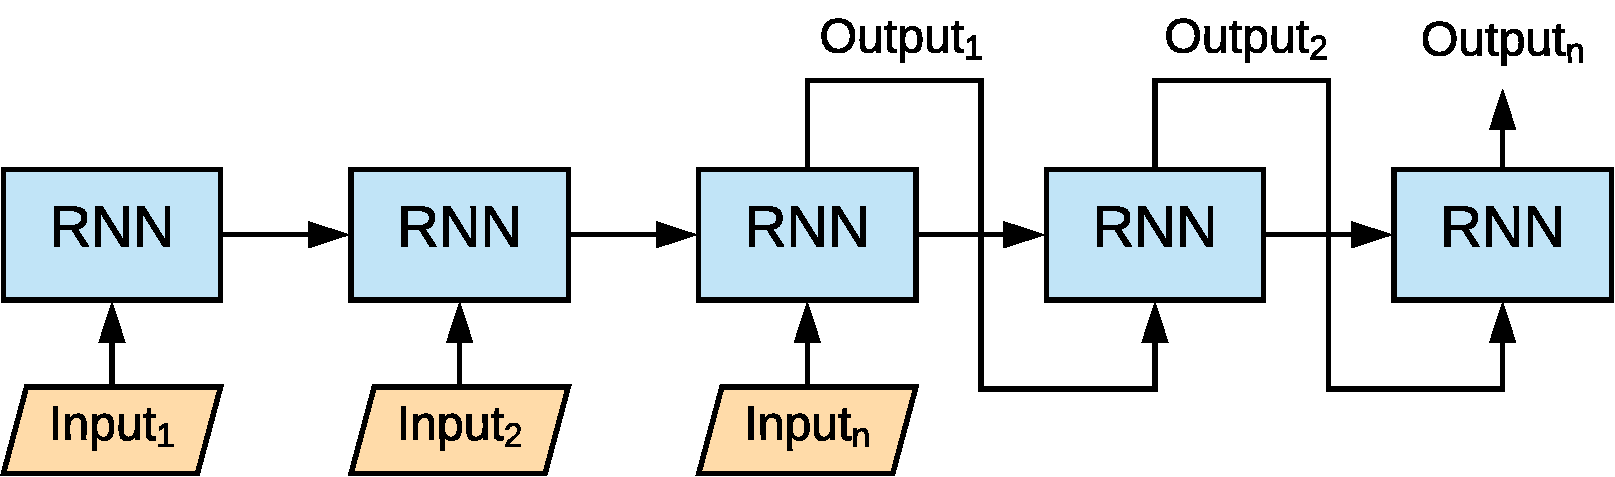
\includegraphics[width=\textwidth]{sample}
\caption{\texttt{do\_sample}}
\bigskip
\end{subfigure}
\begin{subfigure}{.8\textwidth}
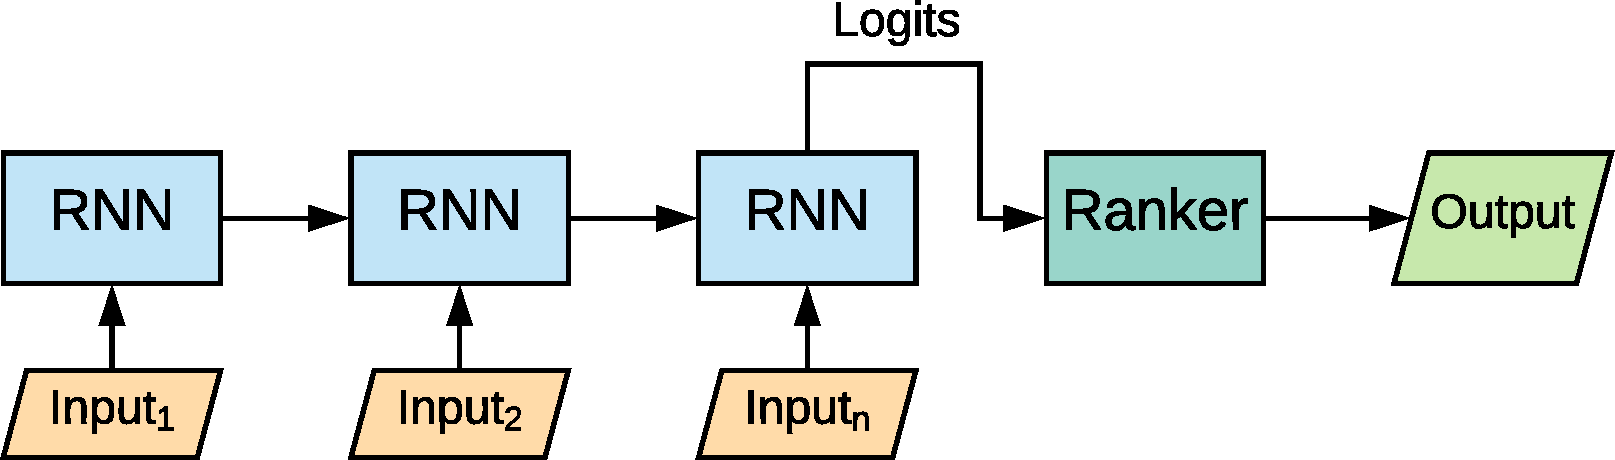
\includegraphics[width=\textwidth]{rank}
\caption{\texttt{do\_rank}}
\bigskip
\end{subfigure}
\begin{subfigure}{.8\textwidth}
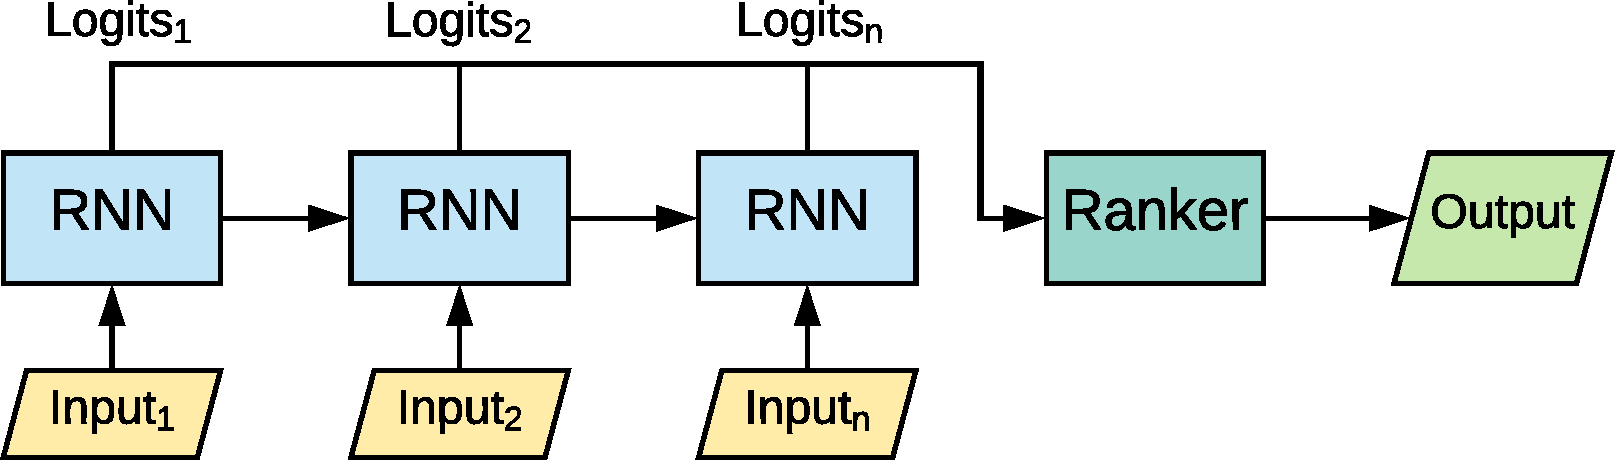
\includegraphics[width=\textwidth]{summed}
\caption{\texttt{do\_summed\_rank}}
\end{subfigure}
\caption[Strategies for generating track predictions]{Our three strategies for generating track predictions.}
\label{rnn:fig:predictions}
\end{figure}

\section{Title2Rec}
\label{rnn:sec:t2r}

Title2Rec recommends tracks taking as input the playlist title, following the procedure illustrated in Figure~\ref{rnn:fig:t2r_rec}. The title is translated into a vector $p_{t2r}$, named title embedding, computed by applying the strategy described in Section~\ref{rnn:sec:title_embs} to the playlists defined in the MPD dataset.

Given a new seed playlist, we compute its title embedding in the same way. Then, we select a subset $P$ including the top-300 most similar playlists to the given one by comparing its embeddings with $p_{t2r}$ using the cosine similarity. Finally, the required number of tracks are selected among the ones available in $P$. The tracks have been ordered to ensure that the most popular ones in $P$ are placed at the top of the list.

\begin{figure}
\centering
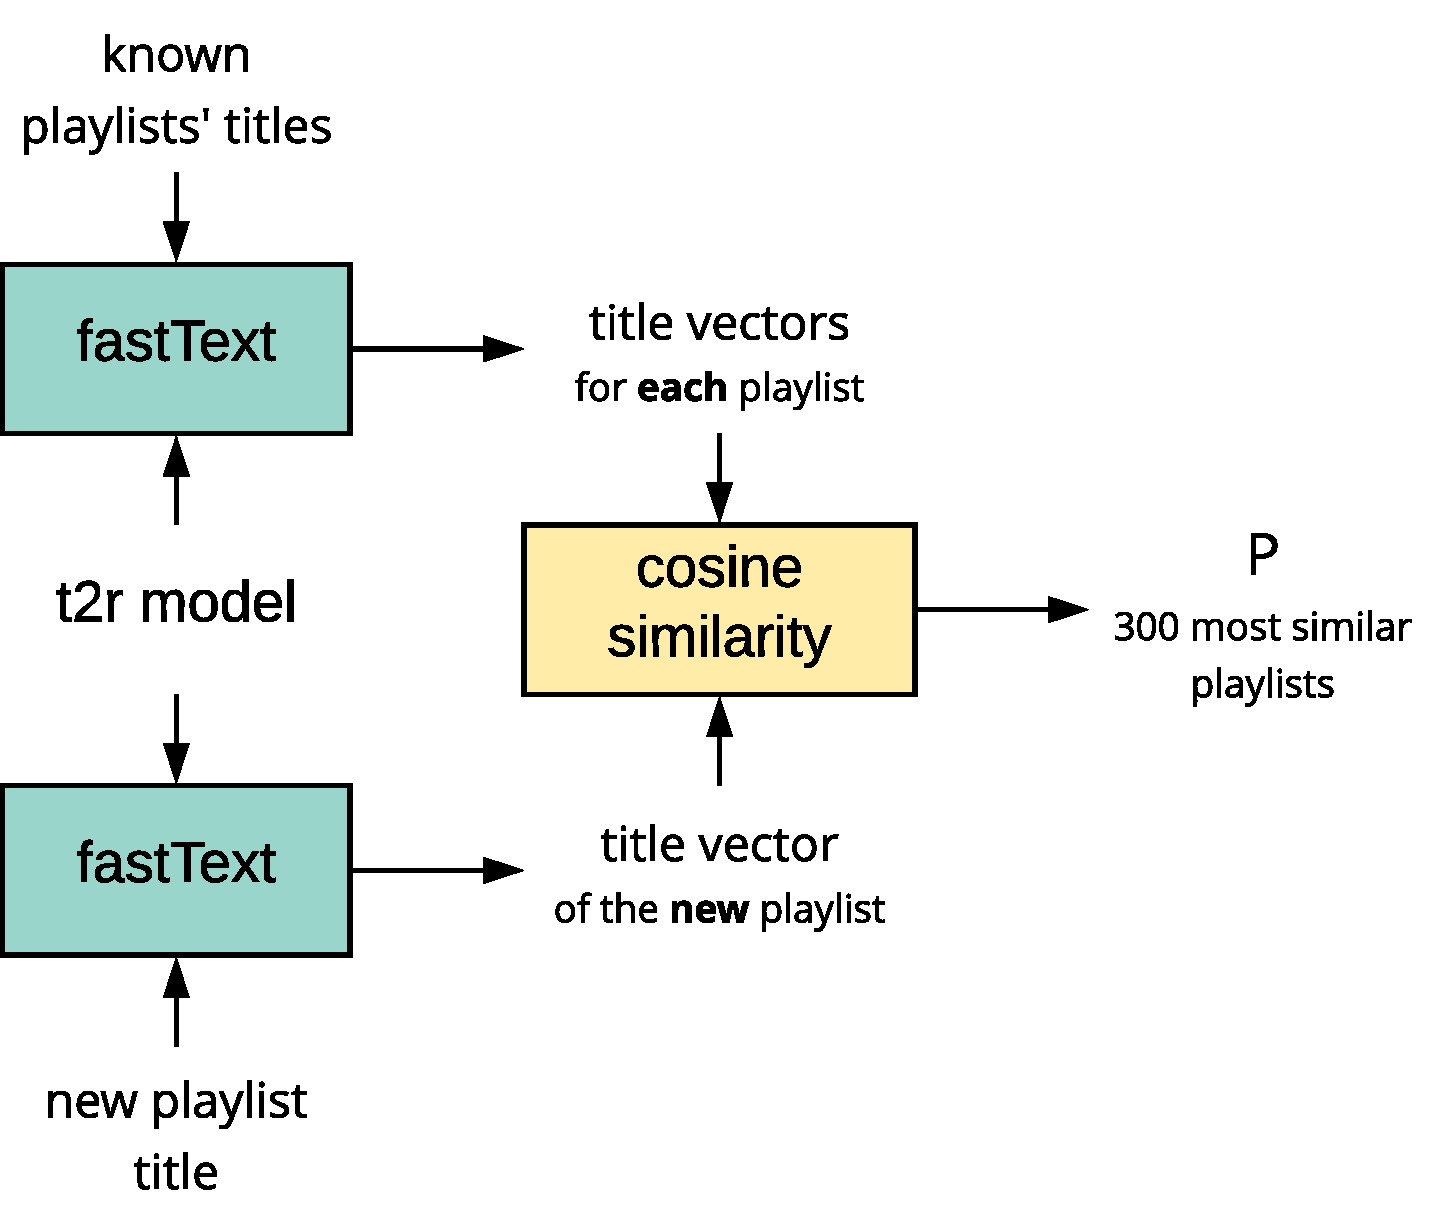
\includegraphics[width=.75\textwidth]{t2r_rec}
\caption[Title2Rec algorithm]{The Title2Rec algorithm compares the fastText representation of the title of a seed playlist to the known ones using the cosine similarity.}
\label{rnn:fig:t2r_rec}
\end{figure}

\section{Optimization}
\label{rnn:sec:optimization}

In the following, we describe the empirical evaluations conducted with the purpose of optimizing the configuration of the RNN, Title2Rec, and the ensemble.

\subsection{RNN Optimization}
\label{rnn:sec:rnn-opt}

For optimizing the hyper-parameters of the RNN, we executed a grid search on a down-sampled version of the MPD dataset containing 100,000 playlists. We considered the following parameters:

\begin{itemize}
\item optimizer: $opt = \{Gradient,\ RMSProp,\ ADAM\}$
\item learning rate: $lr = \{1,\ 0.5,\ 0.1,\ 0.01\}$
\item number of steps: $ns = \{10,\ 20\}$
\item hidden layer size: $hl = \{50,\ 100\}$ 
\end{itemize}

For each configuration $(opt,\ lr,\ ns,\ hl)$, we trained the RNN model and we measured its perplexity on a validation set consisting of 1,000 playlists. Furthermore, we measured its R-Precision, nDCG, and Click metrics as defined in the challenge rules on a separate test set of the same size. The validation and test sets used for optimization purposes contain playlists with the first 5 tracks available as the initial seed, while the others are hidden.

We considered a total of 48 possible configurations: the values of perplexity of the most significant ones are reported in Table~\ref{rnn:tab:rnn_opt}. Perplexity measures the `surprise' of the probabilistic model in observing the data and it is defined as $s^{L}$ where $L$ is the cross-entropy loss function. Thus, lower values of perplexity corresponds to better models. We observe that, when the hidden size is fixed, the best performing optimizer is ADAM. Furthermore, increasing the number of steps reduces the perplexity of the RNN, but it does not have a significant effect on the R-Prec.

Finally, because of time constrains, we selected the configuration $(ADAM,\allowbreak\ 1,\allowbreak\ 10,\allowbreak\ 50)$ as the optimal one, despite its higher perplexity: in fact, we empirically observed that a smaller hidden size results in a shorter training duration.

\begin{table}
\centering
\begin{tabular}{@{}lllllll@{}}
\toprule
Optimizer & L.R. & Steps & Hidden  & ppl     & Time & R-Prec. \\ \midrule
ADAM      & 1    & 20    & 100     & 1357.04 & 3:29 & 0.1739  \\
ADAM      & 1    & 10    & 100     & 1482.86 & 3:39 & 0.1742  \\
Gradient  & 1    & 10    & 100     & 1693.96 & 3:32 & 0.1566  \\
ADAM      & 1    & 10    & 50      & 1716.92 & 2:30 & 0.1745  \\
Gradient  & 1    & 10    & 50      & 2005.54 & 2:25 & 0.1543  \\ \bottomrule
\end{tabular}
\caption[Results of the RNN models]{The results of the most significant RNN models. `L.R.' stands for learning rate, `Steps' for the number of time steps, `Hidden' for the size of the hidden layer, `ppl' stands for perplexity, `Time' is the training time in hours:minutes.}
\label{rnn:tab:rnn_opt}
\end{table}

We evaluated in a controlled setting all the strategies for generating the recommended tracks described in Section~\ref{rnn:sec:generation}. We observed that, independently from other hyper-parameters, the technique called \textit{do\_summed\_rank} systematically achieved better results than the other ones in all the metrics considered. For this reason, we selected this algorithm as our track generation strategy.

Finally, we analyzed the effects on the evaluation metrics of the different categories of features extracted from the lyrics as defined in Section~\ref{rnn:sec:lyrics}, and we selected the groups emotion and fuzzy as the most performing ones.

\subsection{Title2Rec Optimization}
In order to improve the performances of Title2Rec, we worked on different parts of the pipeline. Each optimization has been tested by running the algorithm on a validation set of 1,000 playlists. Then, only the edits that improved the scores with respect to the non-optimized version have been kept in the final version.

We applied a pre-processing on each single title that performed a series of tasks:

\begin{itemize}
\item lowercasing;
\item detecting and separating emoji from words;
\item separating the skin code from the emoji;
\item detecting and separating emoticons from words;
\item transforming space-separated single letters into words (e.g. ``\textit{w o r k o u t}'' becomes ``\textit{workout}'';
\item remove `\#' from hashtags.
\end{itemize}

Other tasks that have been tested with no improvements are:

\begin{itemize}
\item detecting and separating punctuation from words;
\item removing stop words;
\item removing all spaces.
\end{itemize}

The latter point has been partially exploited because we noticed an improvement in the results by including in the corpus both versions of the title, that is keeping the spaces (as in ``green day'') and removing them (``greenday'').

Another optimization step included the usage of different parameters for executing the pipeline. The clustering phase have been tested with different values of $k$ (the number of clusters in output for the K-means algorithm). The value of 500 gives better results than smaller and bigger ones, which produce clusters that are respectively less specialized and less populated. The fastText training has been run with 5 epochs, a learning rate of 0.1 and different loss functions (ns, hs, \textit{softmax}), window sizes (3, \textit{5}, 10). The values in italics represent the best results.

The ordering by popularity described in Section~\ref{rnn:sec:t2r} has been modified so that the impact of each playlist is proportional to the similarity of its title to the seed. In other words, a track has a higher chance to be recommended if it is included in a large number of playlists in $P$ and if most of them are among the top ones more similar to the seed.

Finally, some improvements come from the inclusion of the playlist descriptions in the training. On the whole set of descriptions in the MPD dataset, we compute a TF-IDF model. Thanks to this, we are able to extract a set of keywords for each description by selecting the three words with the highest score. These keywords are added to the documents used to build the clusters. The contribution of the description is null when the playlist does not include any.

\subsection{Ensemble Optimization}

We studied the performance of the ensemble by applying a combination without repetition sampling of different runs for each of the tracks, namely main and creative, and for different groups of runs. In detail, given $n$ the total number of runs, and $k$ the grouping factor, we devised a number of $\frac{n!}{k!(n-k!)}$, where we varied $k=1,\dots,n-1$. We then selected the best performing configuration for both the main and the creative tracks by optimizing the three metrics used for the final ranking. These configurations are reported in Section~\ref{rnn:sec:results}.

\section{Experimental Results}
\label{rnn:sec:results}

In order to evaluate the effectiveness of our approach, we have divided the official MPD dataset in a training, a validation, and a test set. The validation and the test set contain 10,000 playlists each, that is the 1\% of the original dataset. These playlists have been selected according to the characteristics of the MPD provided by Spotify.\footnote{\url{https://recsys-challenge.spotify.com/challenge_readme}} Thus, the validation and test playlists are divided into 10 different categories: each of them defines a peculiar way of hiding some information during the testing phase, i.e. the number of seed tracks or their order.

Furthermore, we have implemented an evaluation tool that computes on our split the same metrics that are described in the challenge rules. Following this approach, it is possible to inspect the evaluation results for each category of the test set separately. As expected, the category containing playlists with only their title and no tracks proved to be the most difficult one to address.

Table~\ref{rnn:tab:approaches} contains the results obtained on our test set by Title2Rec, Word2Rec, and the RNNs trained with different optimizers and input vectors. Word2Rec corresponds to the word2vec model trained on sequences of tracks as described in Section~\ref{rnn:sec:track_embs} and used to generate predictions directly by looking up the 500 most similar tracks to the seeds. All the neural models, but the first two, were trained with the optimal configuration described in Section~\ref{rnn:sec:rnn-opt}. These models are computationally demanding: the training phase lasted more than three days per epoch. The numbers 300 and 400 represent the dimensionality of the input vectors: the 300 models were trained without the title embeddings, while the 400 ones also exploit the fastText model described in Section~\ref{rnn:sec:title_embs}. All the RNNs that include the features extracted from the lyrics were trained with input vectors of dimensionality higher than 400.

\begin{table}
\centering
\begin{tabular}{@{}llllll@{}}
\toprule
Approach    & Optimizer & Epoch & R-Prec.     & nDCG   & Click   \\ \midrule
Title2Rec   & -         & -     & 0.0837      & 0.1260 & 12.007  \\
Word2Rec    & -         & -     & 0.0963      & 0.1444 & 8.4322  \\
RNN 300     & Gradient  & 1     & 0.1417      & 0.1621 & 4.1902  \\
RNN 300     & Gradient  & 2     & 0.1500      & 0.1656 & 3.9433  \\
RNN 300     & ADAM      & 1     & 0.1557      & 0.1702 & 3.9213  \\
RNN 300     & ADAM      & 2     & 0.1457      & 0.1672 & 4.4224  \\
RNN 400     & ADAM      & 1     & 0.1572      & 0.1708 & 3.9340  \\
RNN 400     & ADAM      & 2     & 0.1520      & 0.1694 & 4.1307  \\
RNN Emotion & ADAM      & 1     & 0.1556      & 0.1702 & 4.0101  \\
RNN Emotion & ADAM      & 2     & 0.1500      & 0.1680 & 4.3594  \\
RNN Fuzzy   & ADAM      & 1     & 0.1555      & 0.1698 & 3.9950  \\
RNN Fuzzy   & ADAM      & 2     & 0.1503      & 0.1683 & 4.3456  \\ \bottomrule
\end{tabular}
\caption[Results of different approaches]{Experimental results of different approaches on our test set.}
\label{rnn:tab:approaches}
\end{table}

Table~\ref{rnn:tab:ensemble} lists the results computed on our test set for the best performing configurations in the two tracks of the challenge. The models combined in the ensemble are the following:

\begin{description}
\item[Main track] RNN 300 (Gradient; Epoch 1 and 2), RNN 300 (ADAM; Epoch~1 and 2), and RNN 400 (Epoch 1 and 2).
\item[Creative track] RNN 300 (Gradient; Epoch 1 and 2), RNN 300 (ADAM; Epoch~1 only), RNN 400 (Epoch 1 and 2), RNN Emotion (Epoch 1 and 2), and RNN Fuzzy (Epoch 1 and 2).
\end{description}

\begin{table}
\centering
\begin{tabular}{@{}llll@{}}
\toprule
Track    & R-Precision & nDCG   & Click  \\ \midrule
Main     & 0.1611      & 0.1710 & 3.6349 \\
Creative & 0.1634      & 0.1717 & 3.5964 \\ \bottomrule
\end{tabular}
\caption[Results of the ensemble]{Experimental results of the ensemble on our test set.}
\label{rnn:tab:ensemble}
\end{table}

\section{Conclusion}
\label{rnn:sec:conclusion}

Completing automatically playlists with tracks contained in the MPD dataset is a particularly difficult task due to the dataset dimension and the variety of playlists generated by numerous users having different likes and behaviors bringing great diversity. In this chapter, we presented the D2KLab recommender system that implements an ensemble approach of multiple learning models differently optimized combined with a Borda count strategy. Each model runs an RNN that exploits a wide range of playlist features such as artist, album, track, lyrics (used for the creative track), title and a so-called Title2Rec that takes as input the title and that is used, as fall-back strategy, when playlists do not contain any track. The approach showed to be robust in such a complex setting demonstrating the effectiveness of learning models for automatic playlist completion.

The experimental analysis brought to further attention three points, namely the generation strategy, complementarity of the learning models, and computing time. The generation strategy has a great impact on the results and it pointed out that a recurrent decoding stage is less performing than using a ranking strategy that weighs the output of each RNN of the encoding stage. The ensemble strategy aggregates different outputs of the learning model runs by pivoting the generated ranking. This has granted a sensible increment in performance, so we plan to study further the complementarity of the runs and to build a learning model to automatically select the best candidates. Finally, the computing time has been a crucial experimental setup element due to the generation of the RNN learning model; we addressed it by creating different sizes of the MPD dataset randomly selected and by optimizing the learning models on the hardware at disposal, becoming another factor of differentiation for shaping a performing submission.
